\section{Filtering}
\label{sec:filtering}

\subsection{Adding a New Filter}
When clicking the 'Add filter' button, a dialog is opened.

\begin{figure}[H]
  \center
    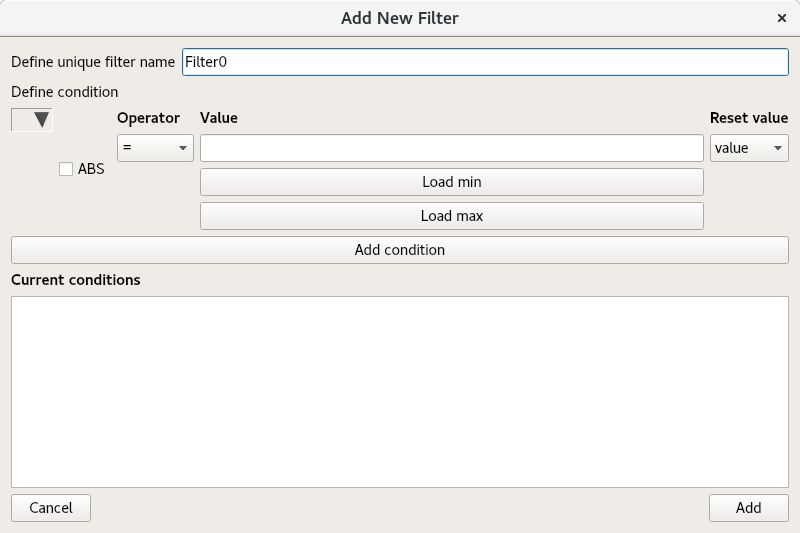
\includegraphics[width=14cm,frame]{../screenshots/filter_add.png}
  \caption{Adding a filter}
  \label{fig:filter_add}
\end{figure}

First, one has to give the filter a new (unique) name. Then, conditions have to be defined and added. A condition consists of a DBO variable, an operator, a value, and a reset value. \\

When the triangular button is clicked, a sub-menu is opened, where one can choose a DBO variable. The selected variable restricts data of all DBOs if it is of type 'Meta', or just data from one DBO if it is not.Additionally, the mathematical operator 'ABS' can be selected. If so, not the value of the variable but the absolute value of the variable is used: 'ABS(var)>value' is equivalent to 'var>value OR var<-value'. \\

An operator can be chosen with the drop-down menu, the supplied operators are common SQL operators.

\begin{table}[H]
  \center
  \begin{tabular}{ | l | l |}
    \hline
    \textbf{Operator} & \textbf{Description} \\ \hline
    = & Equal \\ \hline
    != & Not equal \\ \hline
    > & Greater than \\ \hline
    >= & Greater than or equal \\ \hline
    < & Less than \\ \hline
    <= & Less than or equal \\ \hline
    IN & Matches a value in a comma-separated list \\ \hline
    LIKE & Pattern matching with \% and \_ \\ \hline
    IS & Value NULL: No value exists \\ \hline
    IS NOT & Value NULL: Value exists \\
    \hline
  \end{tabular}
  \caption{SQL operators}
\end{table}

In the 'Value' field one can set a value manually, or load the minimum or maximum values of the selected DBO variable from the database using the 'Load min'/'Load max' buttons . A reset value also has to be supplied, which can be the chosen value or a minimum/maximum value set from the database.  Whenever a database different from the previous one is opened, all filters are reset, since previous values may have become invalid.\\

After a condition is defined, it has to be added using the 'Add condition' button. Existing conditions are
shown in the 'Current conditions' list. Please note that added conditions can not be removed in this dialog,
but have to be removed as described in the Section \nameref{sec:filter_editing}.

\begin{figure}[H]
  \center
    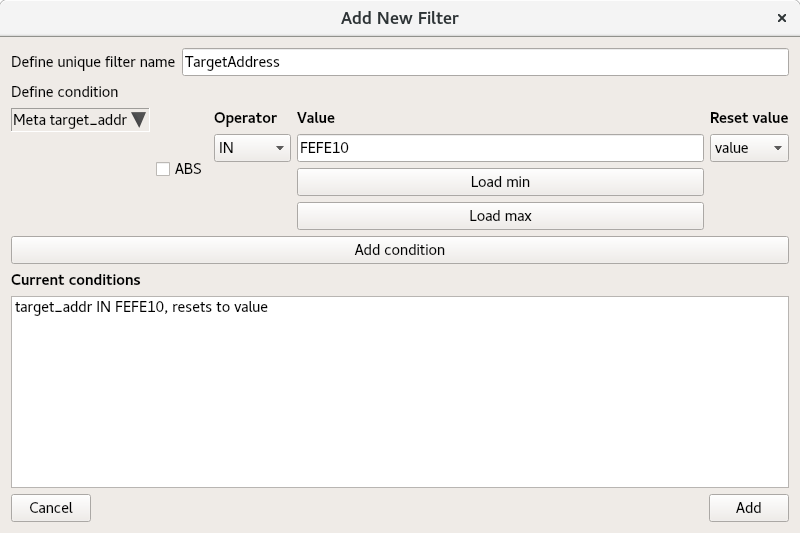
\includegraphics[width=14cm,frame]{../screenshots/filter_add2.png}
  \caption{Filled out filter dialog}
  \label{fig:filter_add2}
\end{figure}

Now the described process can be repeated until a usable filter emerges, which is added using the 'Add'
button. The process of adding a new filter can be canceled by using the 'Cancel' button, which discards all
settings. When added, a new filter shows up immediately in the filter list and is saved to the configuration
for persistence.

\begin{figure}[H]
  \center
    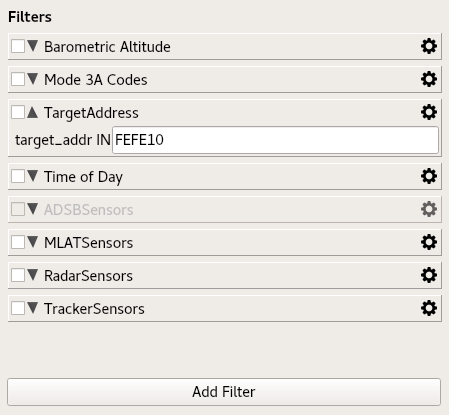
\includegraphics[width=8cm,frame]{../screenshots/filter_add3.png}
  \caption{Filter added}
  \label{fig:filter_add3}
\end{figure}

\subsection{Managing Filters}
\label{sec:filter_management}

By clicking on the gear symbold {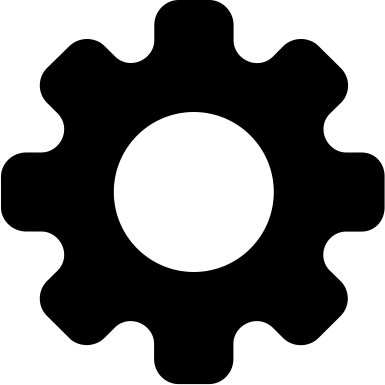
\includegraphics[scale=0.025]{../../data/icons/edit.png}, a menu allows the following operations on the filter:

\begin{itemize}  
\item Reset: Resets the filter to its default values.
\item Edit: Has been disabled and will be added at a later version.
\item Delete: Deletes a filter and permanently removes it from the configuration.
\end{itemize}
 
